\paragraph{User registration}
\begin{center}
\begin{table}[H]
\centering
\begin{tabular}{l|p{0.7\textwidth}}
\textbf{Actors} & Not registered user, Mobile app, Track4Me core App \\
\textbf{Start conditions} & None \\
\textbf{Event flow}  & 


 \begin{minipage}[t] {0.7\textwidth} 
 \begin{itemize}
      \item  not registered user clicks on “Subscribe”
      \item not registered user inserts an username, an email, a Fiscal Code or SSN and a password
      \item The system checks if username is not used by any other user
      \item The system checks if email is not used by any other user
      \item The system checks if Fiscal Code / SSN is valid
      \item The mobile app checks if a compatible smartwatch is connected and has the Smartwatch Data4Help app installed
      \item The system generates a confirmation mail
      \item The user confirms the registration inserting the code received via email 
      \item The system shows a registration complete screen
  \end{itemize}
\end{minipage}
 \\
\textbf{Exit condition} & User information used for registering are stored in the company database \\
\textbf{Exceptions} & 
\begin{minipage}[t] {0.7\textwidth} 
 \begin{itemize}
 
 \item The username is used by another user
\item The email is used by another user
\item The Fiscal Code/SSN is not valid
\item Smartwatch is not compatible
\item Smartwatch has not Data4Help app installed
\end{itemize}
 \end{minipage}\\
\textbf{Goals} & G2 
\end{tabular}

\end{table}
\end{center}


\begin{figure}[H]
  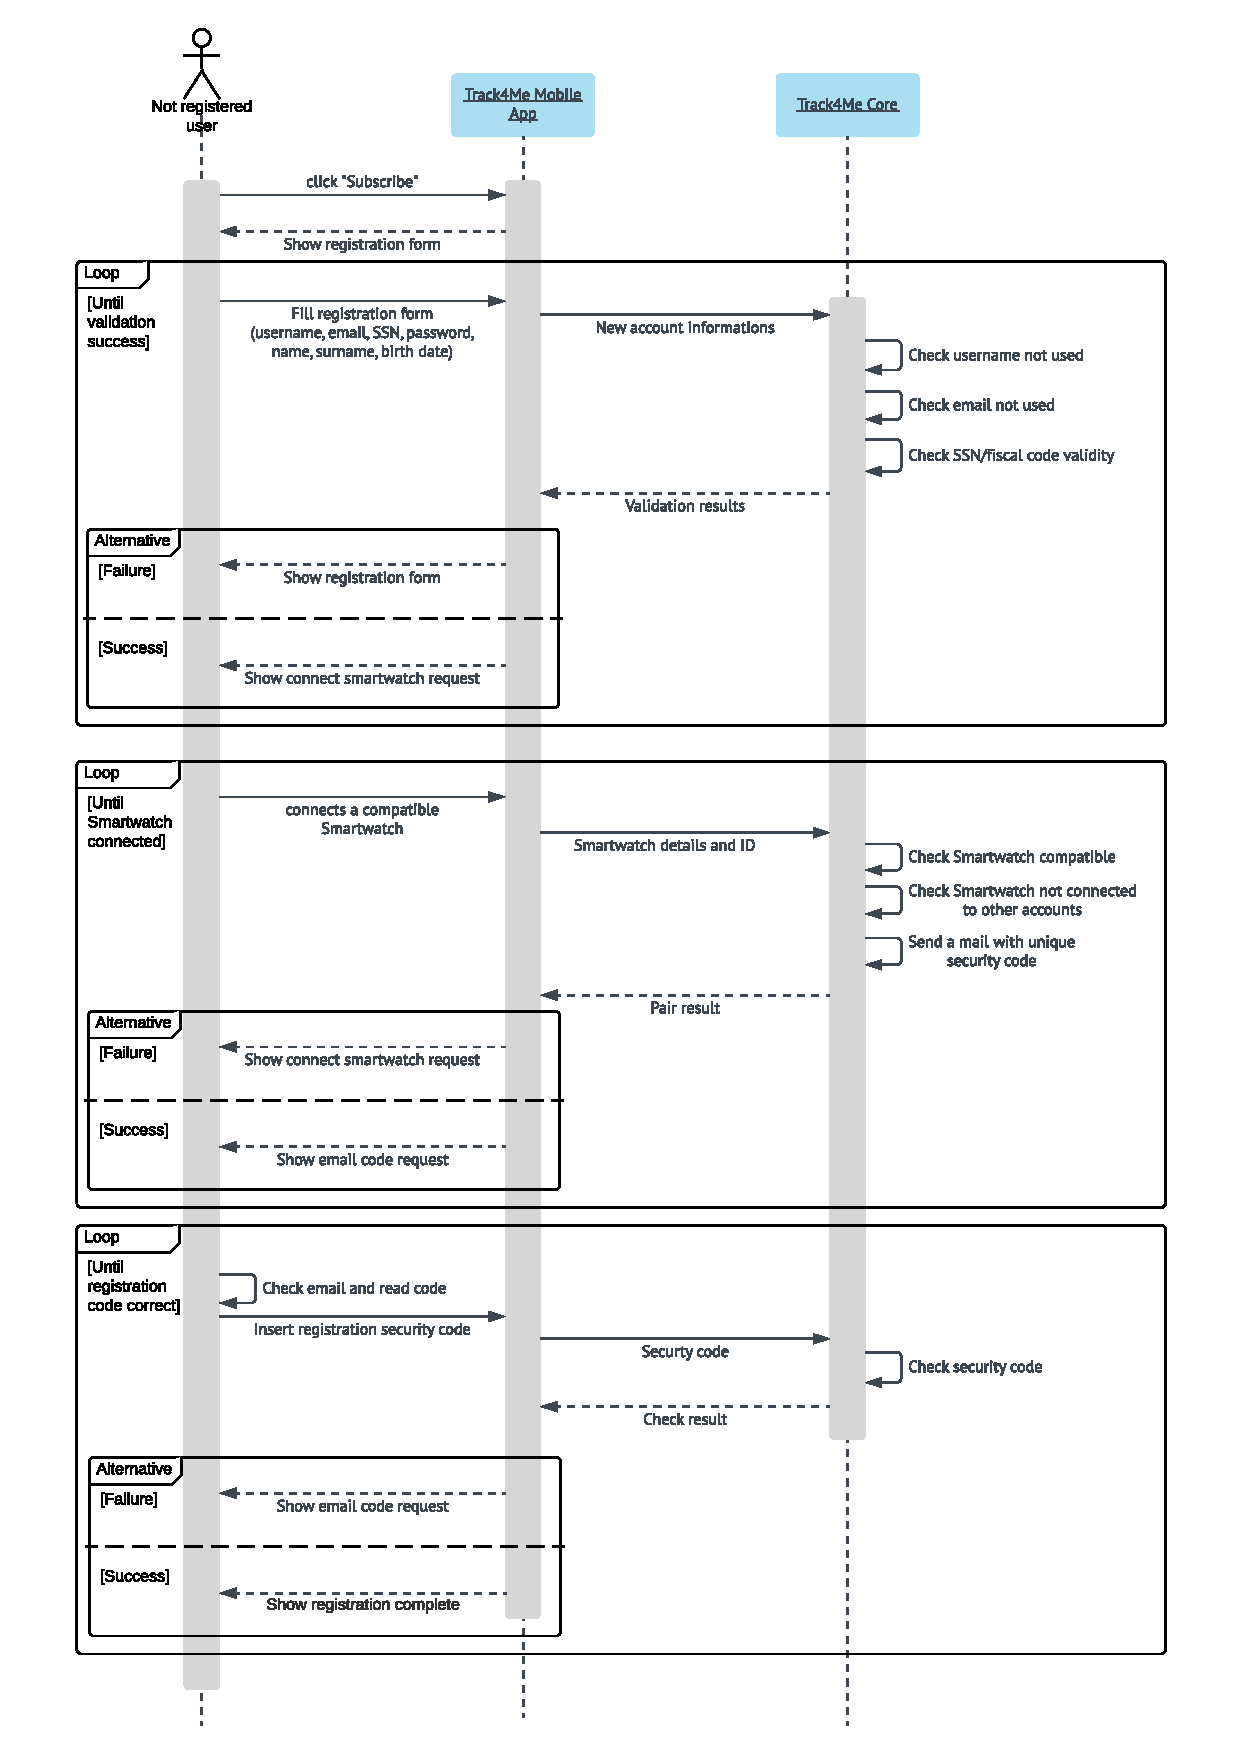
\includegraphics[width=\textwidth,height=\textheight,keepaspectratio]{assets/sequence/UserRegistration.pdf}
  \caption{User registration sequence diagram}
  \label{fig:UserRegistrationSequence}
\end{figure}



\newpage
\paragraph{Consulting of activity history}
\begin{center}
\begin{table}[H]
\centering
\begin{tabular}{l|p{0.7\textwidth}}
\textbf{Actors} & Registered User \\
\textbf{Start conditions} & The user is logged in \\
\textbf{Event flow}  & \begin{minipage}[t]{0.7\textwidth}
    \begin{itemize}
        \item Registered user clicks on “Show past activities” on the Mobile phone
        \item the app shows a screen for searching data information
        \item registered user inserts year, month and the day to search and clicks on the type of data searched
        \item  the system searches for a correspondence in the company database
        \item the system shows a screen showing the required data in a graph
    \end{itemize}
    
\end{minipage}\\ 
    
\textbf{Exit condition} & None \\
\textbf{Exceptions} &  \begin{minipage}[t]{0.7\textwidth}
    \begin{itemize}
        \item The specified day of the calendar is not valid

        \item The specified day of the calendar shows no activities of the user
    \end{itemize}
    
\end{minipage} \\
\textbf{Goals} & \textbf{G1}
\end{tabular}

\end{table}
\end{center}

\begin{figure}[H]
  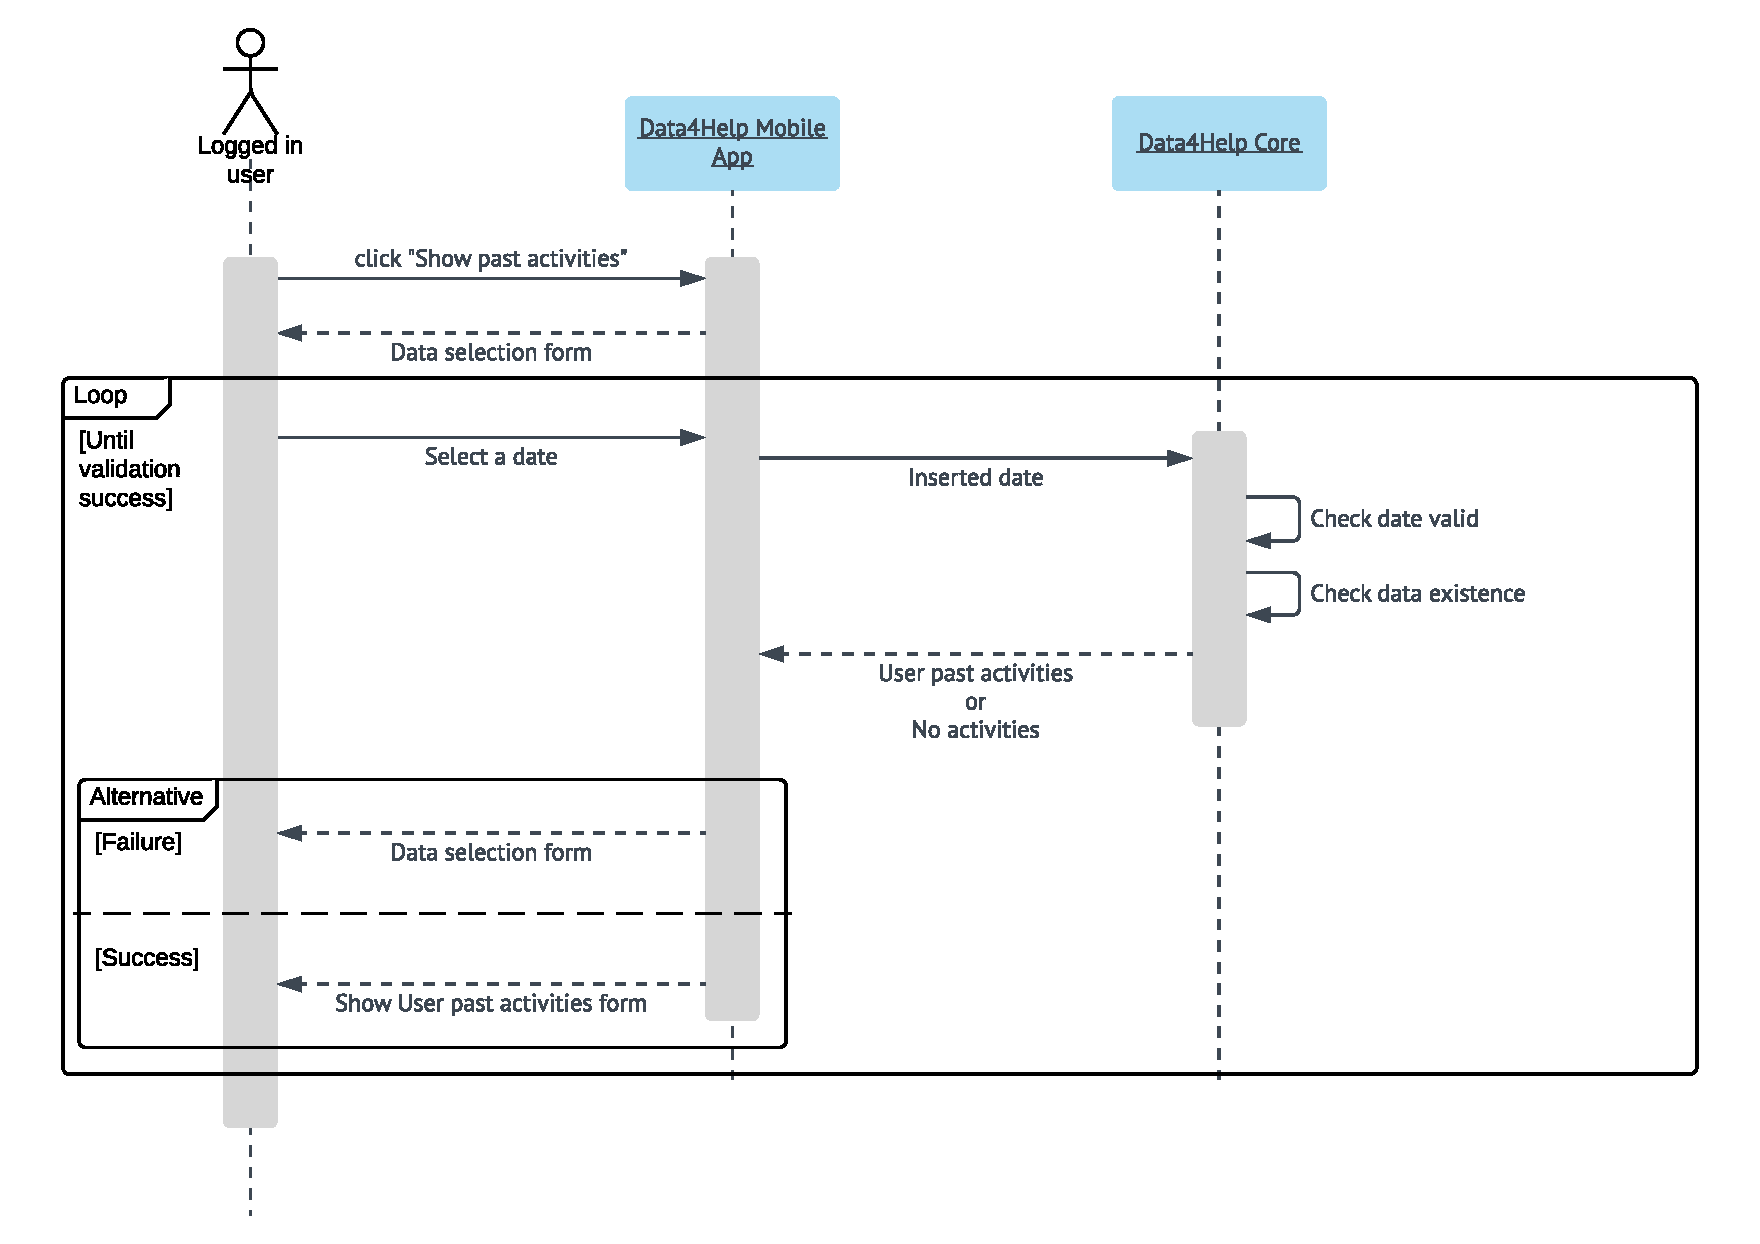
\includegraphics[width=\textwidth,height=\textheight,keepaspectratio]{assets/sequence/ConsultingOfActivityHistory.pdf}
  \caption{Consulting of activity history sequence diagram}
  \label{fig:ConsultingOfActivityHistory}
\end{figure}










\paragraph{Data Synchronization between Smartwatch and Smartphone}
\begin{center}
\begin{table}[H]
\centering
\begin{tabular}{l|p{0.7\textwidth}}
\textbf{Actors} & 
Mobile app, smartwatch app \\
\textbf{Start conditions} & Bluetooth connection enstablished between smartwatch and smartphone \\
\textbf{Event flow}  & \begin{minipage}[t]{0.7\textwidth}
    \begin{itemize}
        \item User turns on Bluetooth of the smartwatch and smartphone


        \item The smartphone requests connection to smartwatch

        \item Smartwatch confirms connection
        \item Smartwatch send data registered in the day 
        \item Smartphone accept data and store locally

    \end{itemize}
    
\end{minipage}\\
\textbf{Exit condition} & Data in the user smartphone is synchronized with data of the smartwatch and stored locally \\
\textbf{Exceptions} & Connection Refused \\
\textbf{Goals} & G1
\end{tabular}

\end{table}
\end{center}

\begin{figure}[H]
  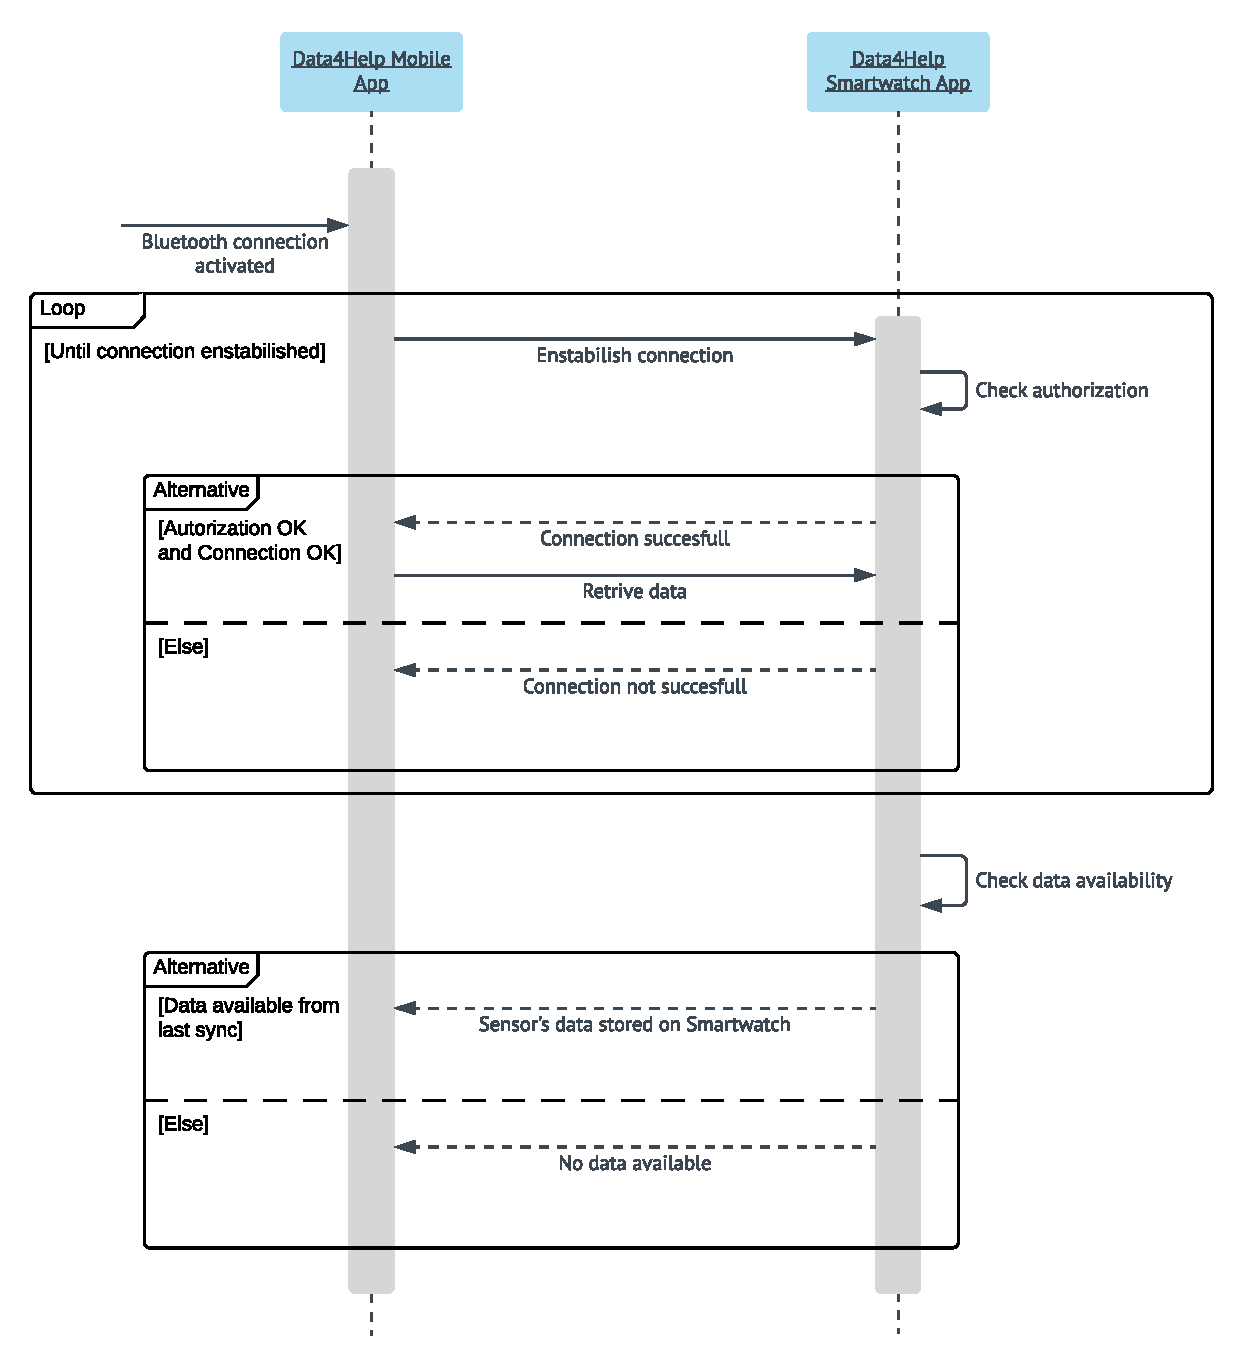
\includegraphics[width=\textwidth,height=\textheight,keepaspectratio]{assets/sequence/DataSynchronizationBetweenSmartwatchAndSmartphone.pdf}
  \caption{Data Synchronization between Smartwatch and Smartphone sequence diagram}
  \label{fig:DataSynchronizationBetweenSmartwatchAndSmartphone}
\end{figure}










\newpage
\paragraph{Company registration}
\begin{center}
\begin{table}[H]
\centering
\begin{tabular}{l|p{0.7\textwidth}}
\textbf{Actors} & Not registered company \\
\textbf{Start conditions} & None \\


\textbf{Event flow}  & \begin{minipage}[t]{0.7\textwidth}
    \begin{itemize}
        \item not registered company clicks on “Subscribe”
\item not registered company inserts a username, an email, a payment method and a password
\item The system checks if email is not used by any other user
\item The system checks if Payment method is valid
\item The system generates a confirmation mail
\item The company confirms the registration click on “Confirm email”
\item The system shows a registration complete screen
    \end{itemize}
    
\end{minipage}\\ 

\textbf{Exit condition} & Company information used for registering is stored in the company database \\
\textbf{Exceptions} & \begin{minipage}[t]{0.7\textwidth}
    \begin{itemize}
        \item The username is used by another company
\item The email is used by another company
\item The Payment method is not valid

    \end{itemize}
    
\end{minipage}\\
\textbf{Goals} & G3 
\end{tabular}

\end{table}
\end{center}

\begin{figure}[H]
  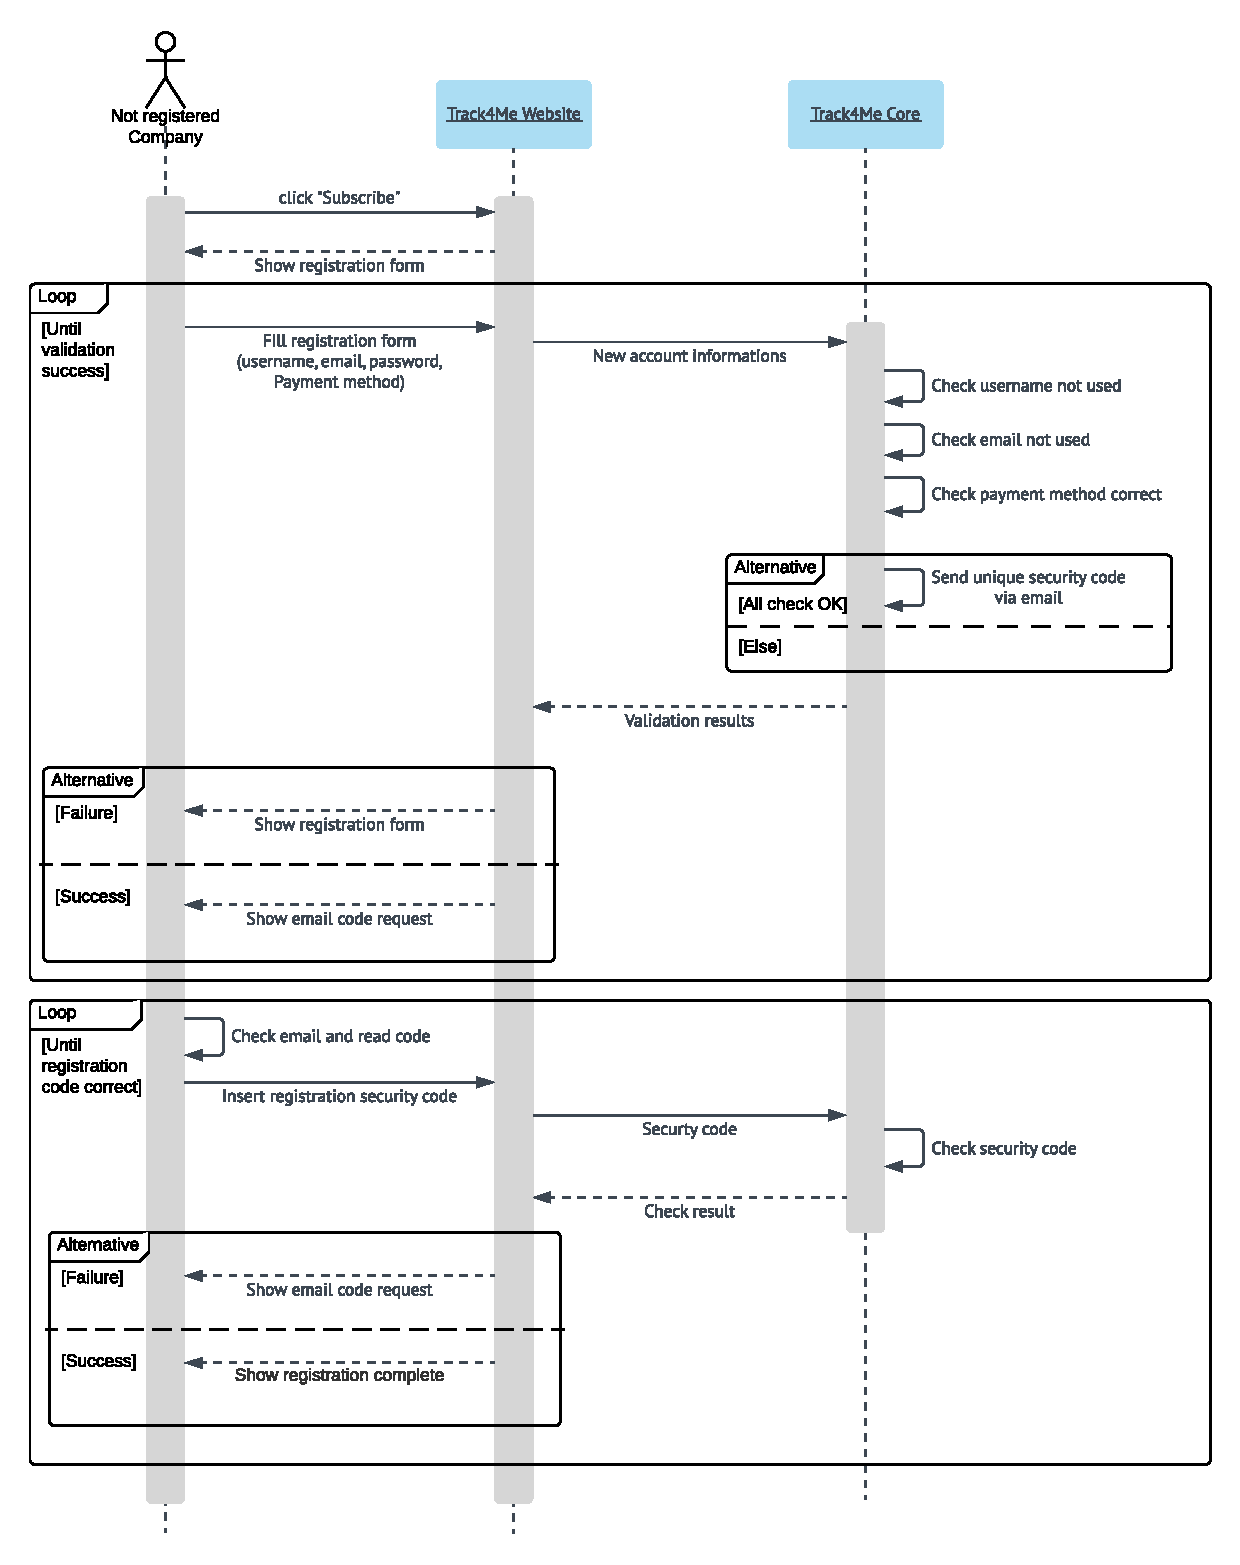
\includegraphics[width=\textwidth,height=\textheight,keepaspectratio]{assets/sequence/CompanyRegistration.pdf}
  \caption{Company registration sequence diagram}
  \label{fig:CompanyRegistration}
\end{figure}











\newpage
\paragraph{Company query search on multiple individuals}
\begin{center}
\begin{table}[H]
\centering
\begin{tabular}{l|p{0.7\textwidth}}
\textbf{Actors} &
Company, WebSite, core component
 \\
\textbf{Start conditions} & None \\
\textbf{Event flow}  &  \begin{minipage}[t]{0.7\textwidth}
    \begin{itemize}
        \item Company clicks on “Start a query” on the website


        \item System checks if the company has query left

        \item System shows the page on the website
        \item Company specifies age of people to search, hours of the day, health parameter filters
 
        \item System validates the request
        \item System send the required data formatted on a pdf page on the website
        \item Company download the data

    \end{itemize}
    
\end{minipage} \\
\textbf{Exit condition} & Query generated as pdf file and stored in the Data4Help database \\
\textbf{Exceptions} & \begin{minipage}[t]{0.7\textwidth}
    \begin{itemize}
        \item No query left for the company type of subscription
        \item Not valid query
    \end{itemize}
    
\end{minipage} \\
\textbf{Goals} & G4
\end{tabular}

\end{table}
\end{center}

\begin{figure}[H]
  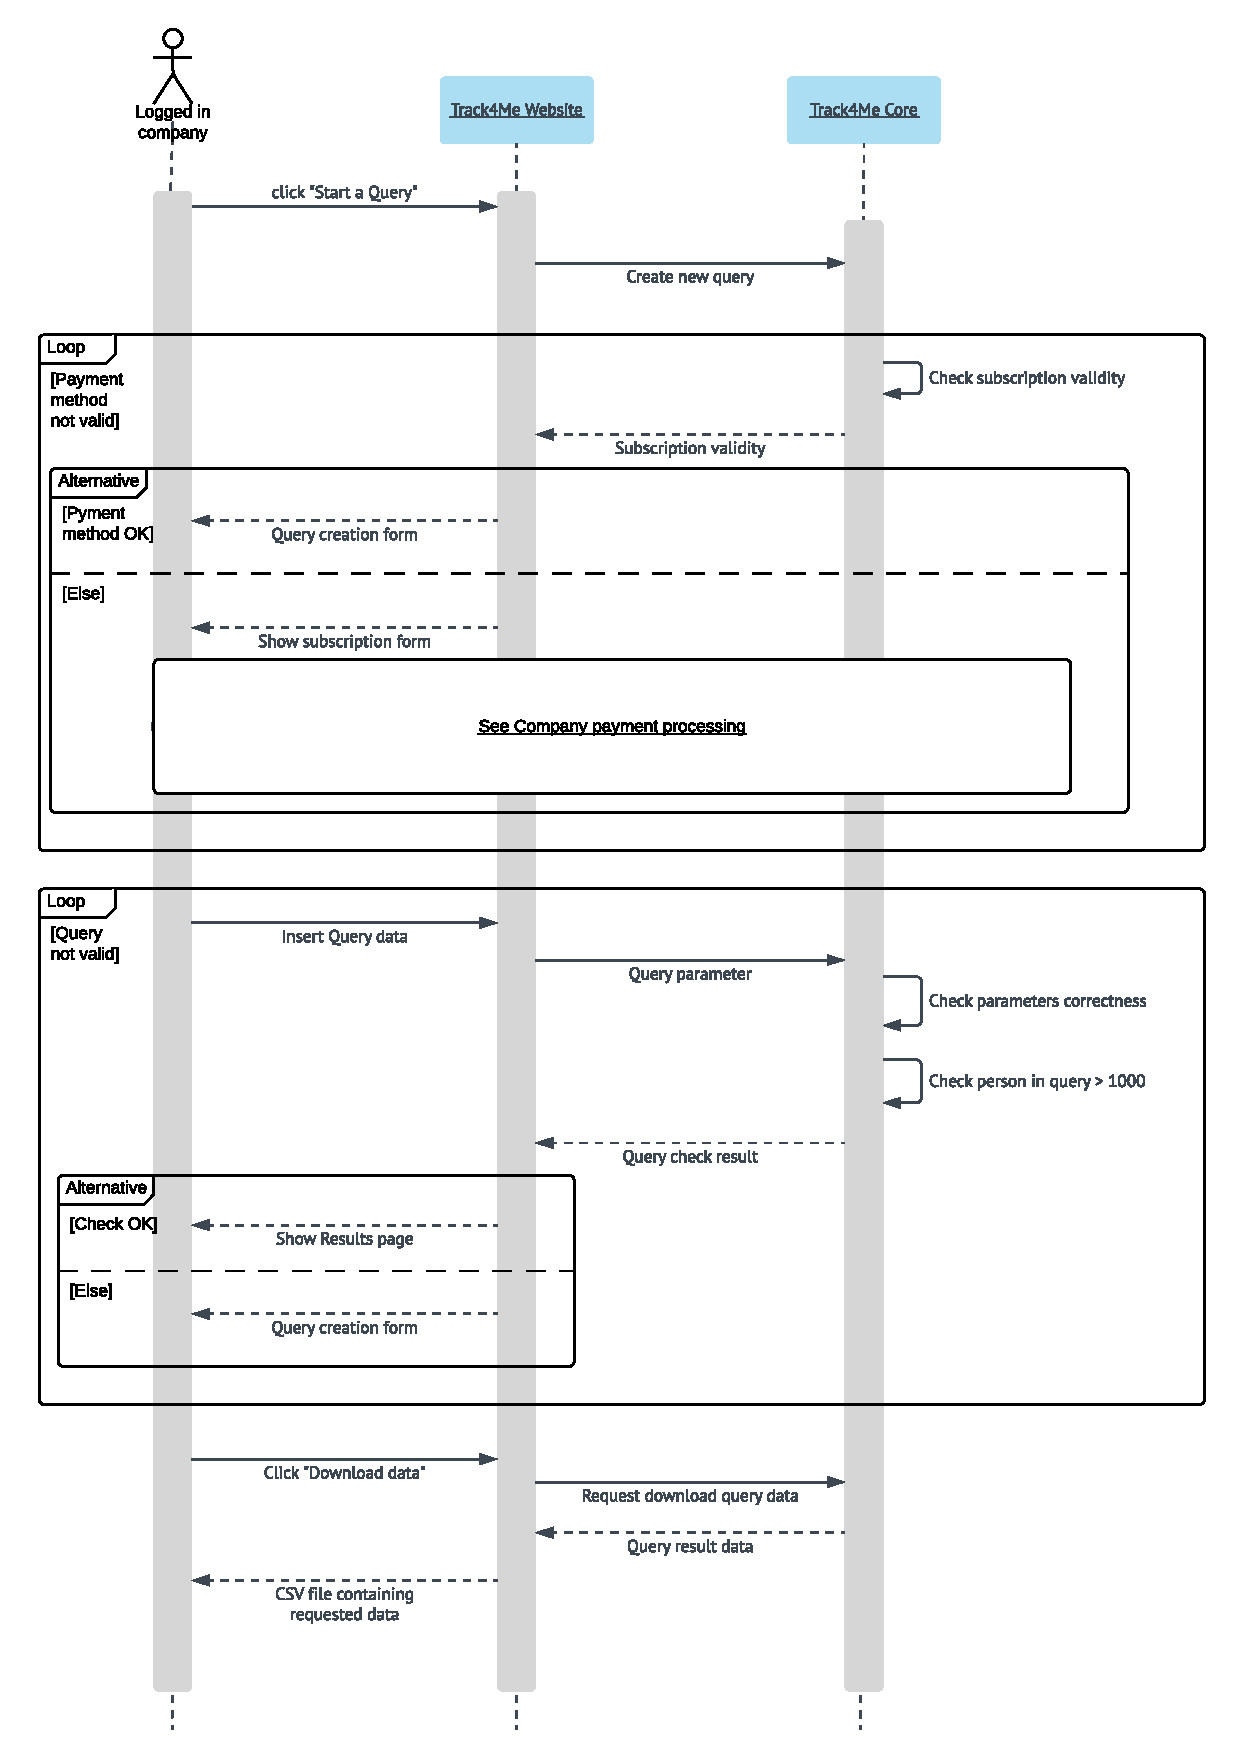
\includegraphics[width=\textwidth,height=\textheight,keepaspectratio]{assets/sequence/CompanyQuerySearchOnMultipleIndividuals.pdf}
  \caption{Company query search on multiple individuals sequence diagram}
  \label{fig:CompanyQuerySearchOnMultipleIndividuals}
\end{figure}
















\newpage
\paragraph{Company request for individual monitoring}
\begin{center}
\begin{table}[H]
\centering
\begin{tabular}{l|p{0.7\textwidth}}
\textbf{Actors} & Company, User, Core component \\
\textbf{Start conditions} & None \\
\textbf{Event flow}  & 

\begin{minipage}[t]{0.7\textwidth}
    \begin{itemize}
        \item Company clicks on add new patient 
\item System checks if the company can add new patients 
\item Company insert the username of the patient 
\item System checks if username exists in the database
\item System send a monitoring request notification to the user 
\item Username clicks on “Accept requests” through the Mobile app notification or through the email notification 
    \end{itemize}
    
\end{minipage}

\\
\textbf{Exit condition} & 
\begin{minipage}[t]{0.7\textwidth}
    \begin{itemize}
       \item System adds information of the monitoring company to the user in the database
\item The system update number of patient left to monitor of the company in the database

    \end{itemize}
    
\end{minipage}
\\
\textbf{Exceptions} & 

\begin{minipage}[t]{0.7\textwidth}
    \begin{itemize}
       \item No new patients left for the company type of subscription
\item Username not found
\item User refuses the request

    \end{itemize}
    
\end{minipage}
\\
\textbf{Goals} & G5 
\end{tabular}

\end{table}
\end{center}

\begin{figure}[H]
  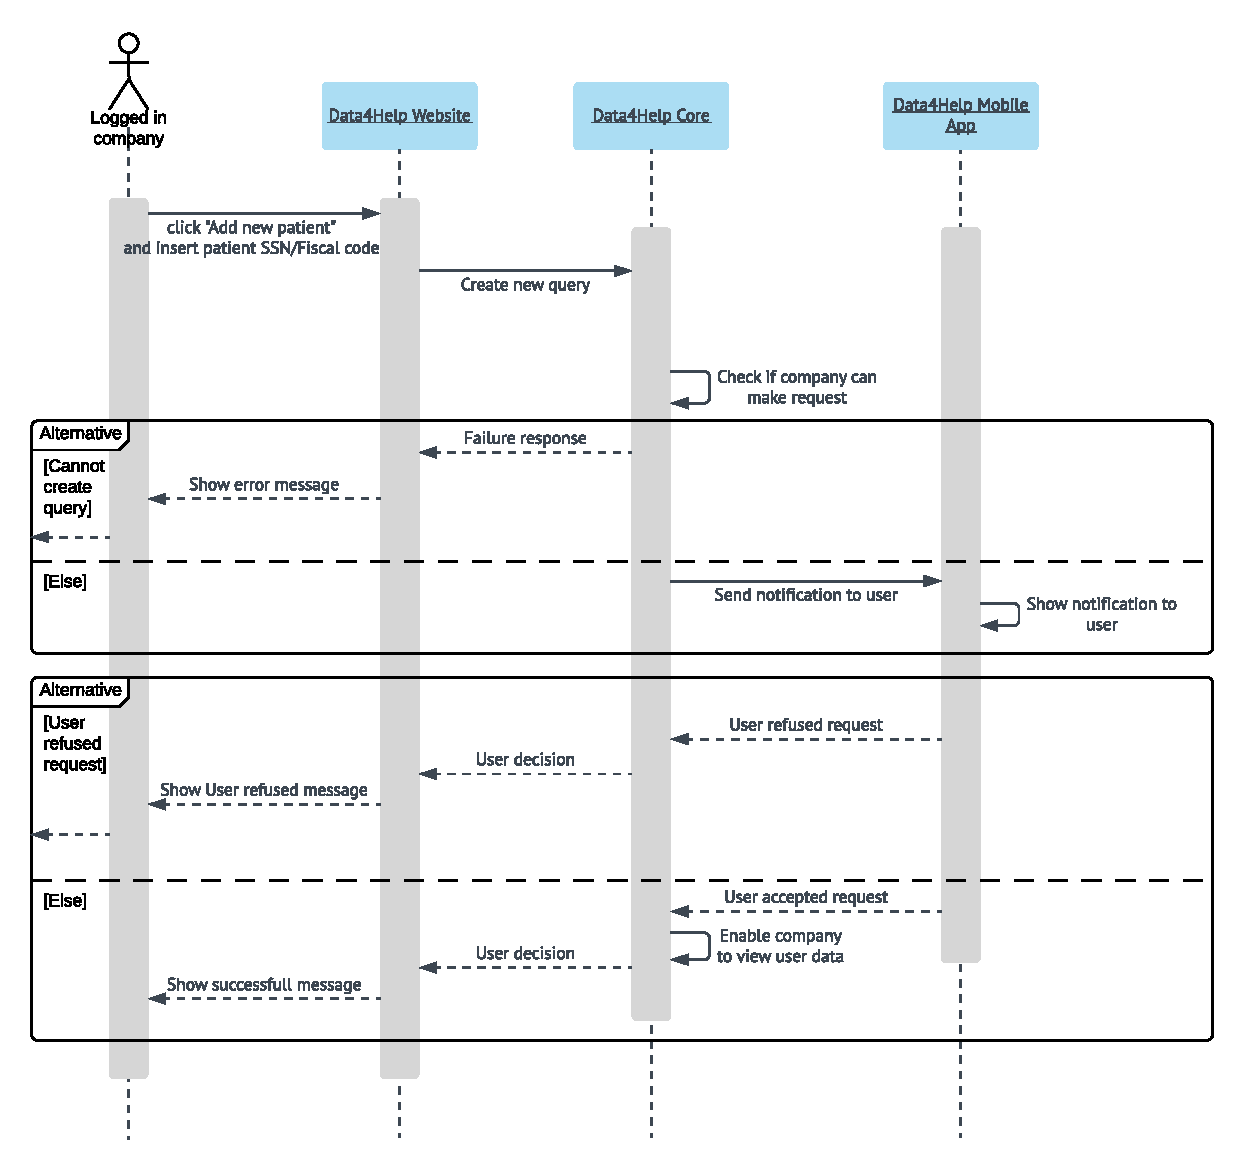
\includegraphics[width=\textwidth,height=\textheight,keepaspectratio]{assets/sequence/CompanyRequestForIndividualMonitoring.pdf}
  \caption{Company request for individual monitoring sequence diagram}
  \label{fig:CompanyRequestForIndividualMonitoring}
\end{figure}
















\newpage
\paragraph{Company consulting of individual data}
\begin{center}
\begin{table}[H]
\centering
\begin{tabular}{l|p{0.7\textwidth}}
\textbf{Actors} & Company, core component \\
\textbf{Start conditions} & None \\
\textbf{Event flow}  & 
\begin{minipage}[t]{0.7\textwidth}
    \begin{itemize}
        \item Company clicks on “See patients information” on the website

\item System shows a page listing all active patients for the company

\item Company clicks on the desired patient name

\item System shows all information of the patient and a menu where to choose a day 

\item Company chooses a day of the calendar from the menu
\item System shows the data of the patient on the specified day

    \end{itemize}
    
\end{minipage}\\
\textbf{Exit condition} & None \\
\textbf{Exceptions} & \begin{minipage}[t]{0.7\textwidth}
    \begin{itemize}
       \item No query left for the company type of subscription
        \item Not valid query

    \end{itemize}
    
\end{minipage} \\
\textbf{Goals} & G5 
\end{tabular}

\end{table}
\end{center}
\begin{figure}[H]
  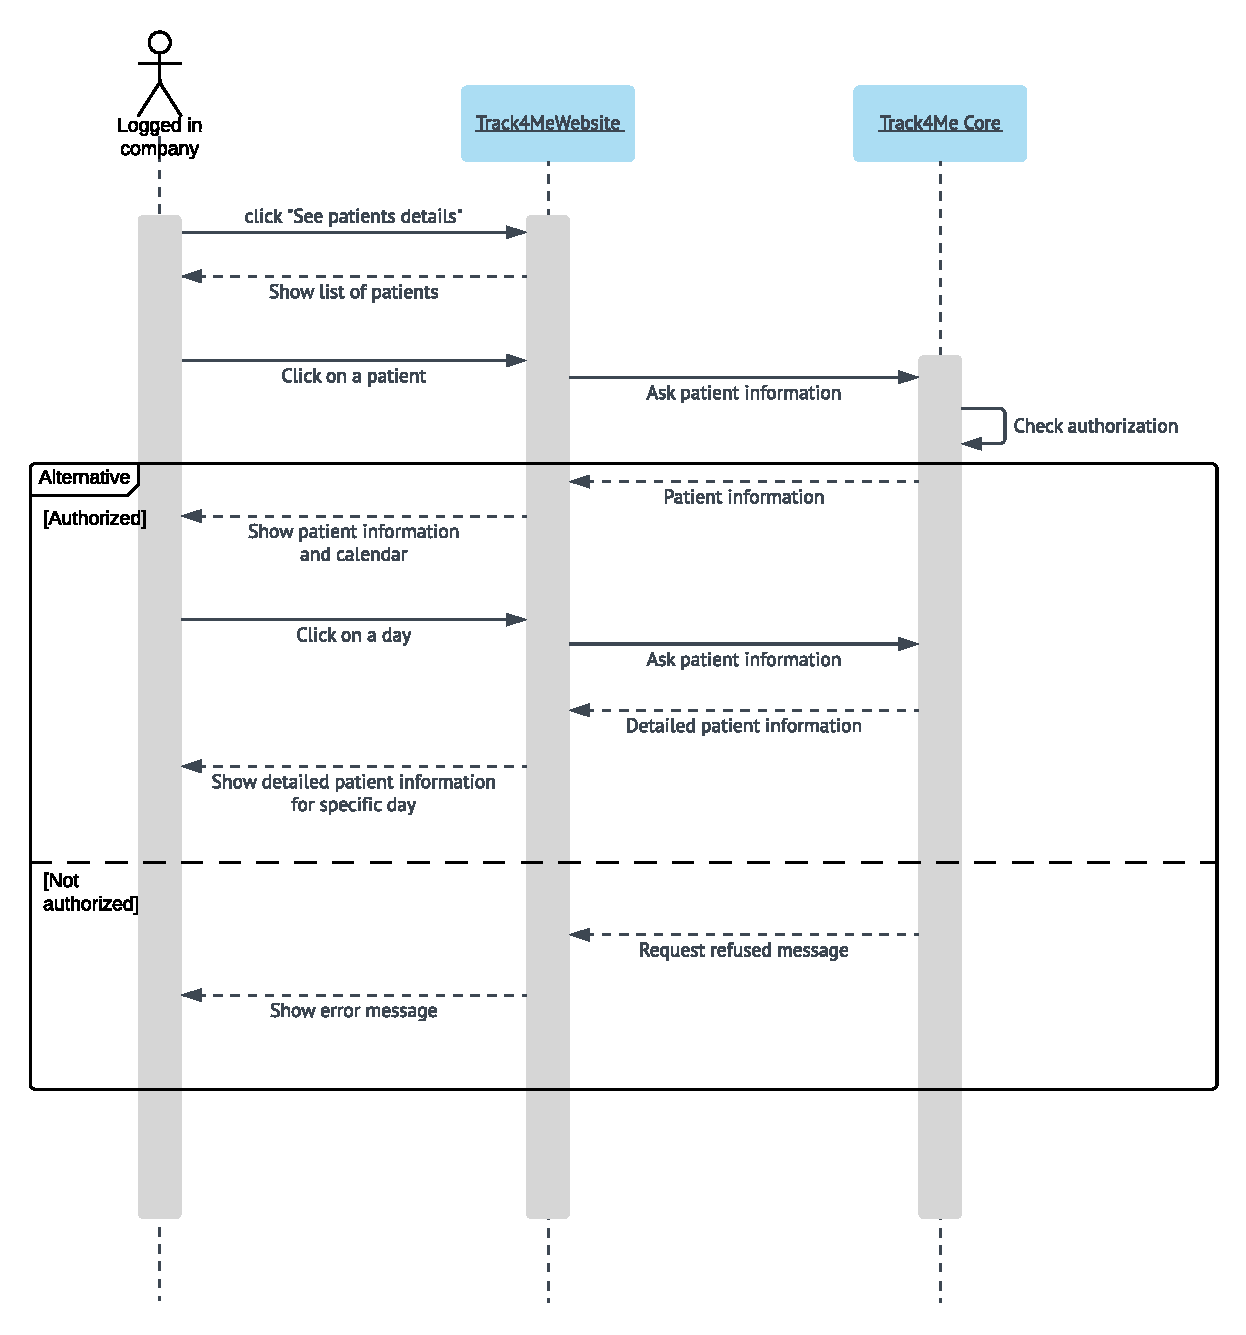
\includegraphics[width=\textwidth,height=\textheight,keepaspectratio]{assets/sequence/CompanyConsultingOfIndividualData.pdf}
  \caption{Company consulting of individual data sequence diagram}
  \label{fig:CompanyConsultingOfIndividualData}
\end{figure}













\newpage
\paragraph{Company payment processing}
\begin{center}
\begin{table}[H]
\centering
\begin{tabular}{l|p{0.7\textwidth}}
\textbf{Actors} & Company, Core component \\
\textbf{Start conditions} & Company purchases a subscription plan \\
\textbf{Event flow}  & \begin{minipage}[t]{0.7\textwidth}
    \begin{itemize}
       \item Company insert the number of the credit card and the CVV
\item System verify the card has enough money
\item The system get the money from the credit card
\item The system show a Successful operation 


    \end{itemize}
    
\end{minipage} \\
\textbf{Exit condition} & The system stored the information of the subscription of the company in the database \\
\textbf{Exceptions} & \begin{minipage}[t]{0.7\textwidth}
    \begin{itemize}
       \item Not enough money
        \item Not valid credit card information
    \end{itemize}
    
\end{minipage} \\
\textbf{Goals} & G6 
\end{tabular}

\end{table}
\end{center}


\begin{figure}[H]
  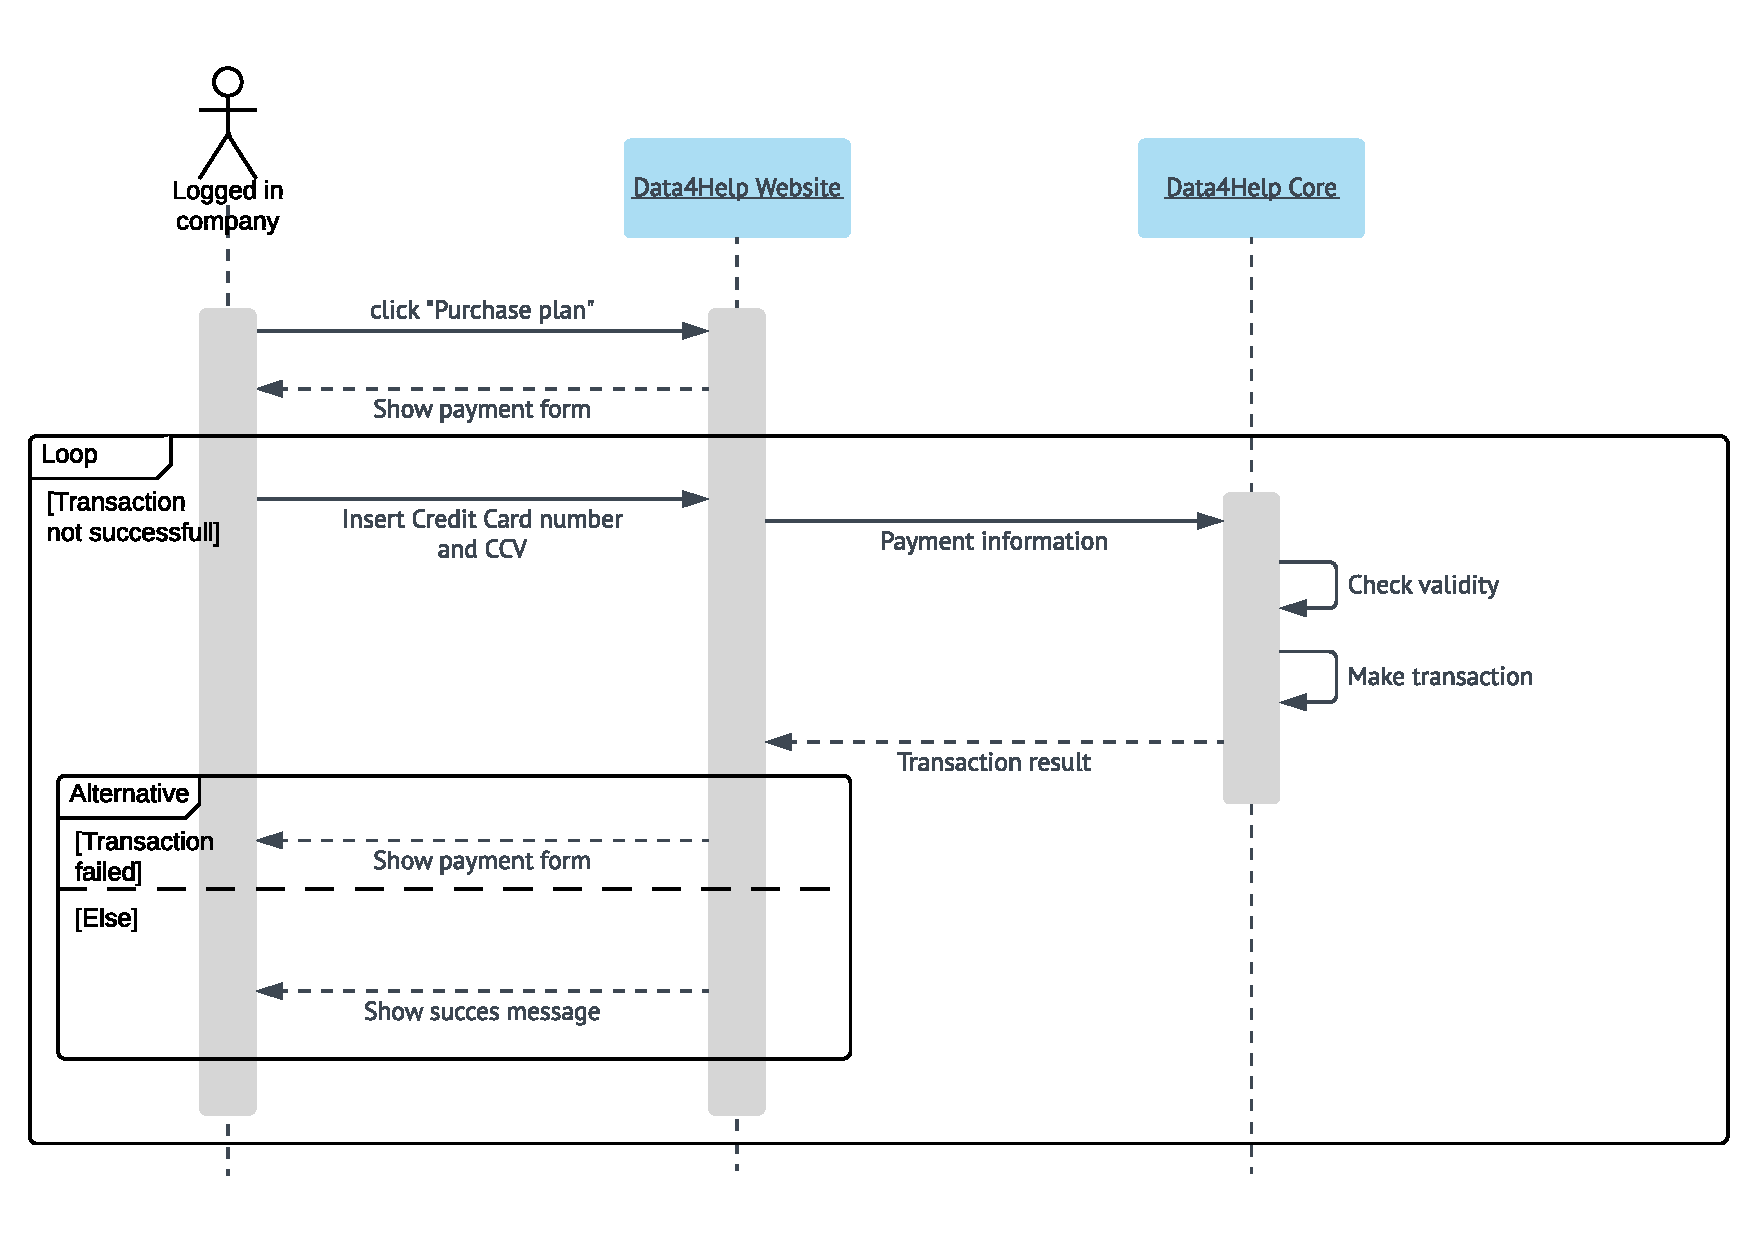
\includegraphics[width=\textwidth,height=\textheight,keepaspectratio]{assets/sequence/CompanyPaymentProcessing.pdf}
  \caption{Company payment processing sequence diagram}
  \label{fig:CompanyPaymentProcessing}
\end{figure}











\newpage
\paragraph{Company receives data of subscribed query}
\begin{center}
\begin{table}[H]
\centering
\begin{tabular}{l|p{0.7\textwidth}}
\textbf{Actors} & 
Company, core component
 \\
\textbf{Start conditions} & Is 0:01 of one month passed after the last data sent of the query \\
\textbf{Event flow}  & \begin{minipage}[t]{0.7\textwidth}
    \begin{itemize}
       \item System retrieve the query information on the database

        \item System compute query on the database
        \item System export a CSV of the data stored
        \item System send the document on the email of the company 


    \end{itemize}
    
\end{minipage} \\
\textbf{Exit condition} & None \\
\textbf{Exceptions} & None \\
\textbf{Goals} & \textbf{G7} 
\end{tabular}

\end{table}
\end{center}

\begin{figure}[H]
  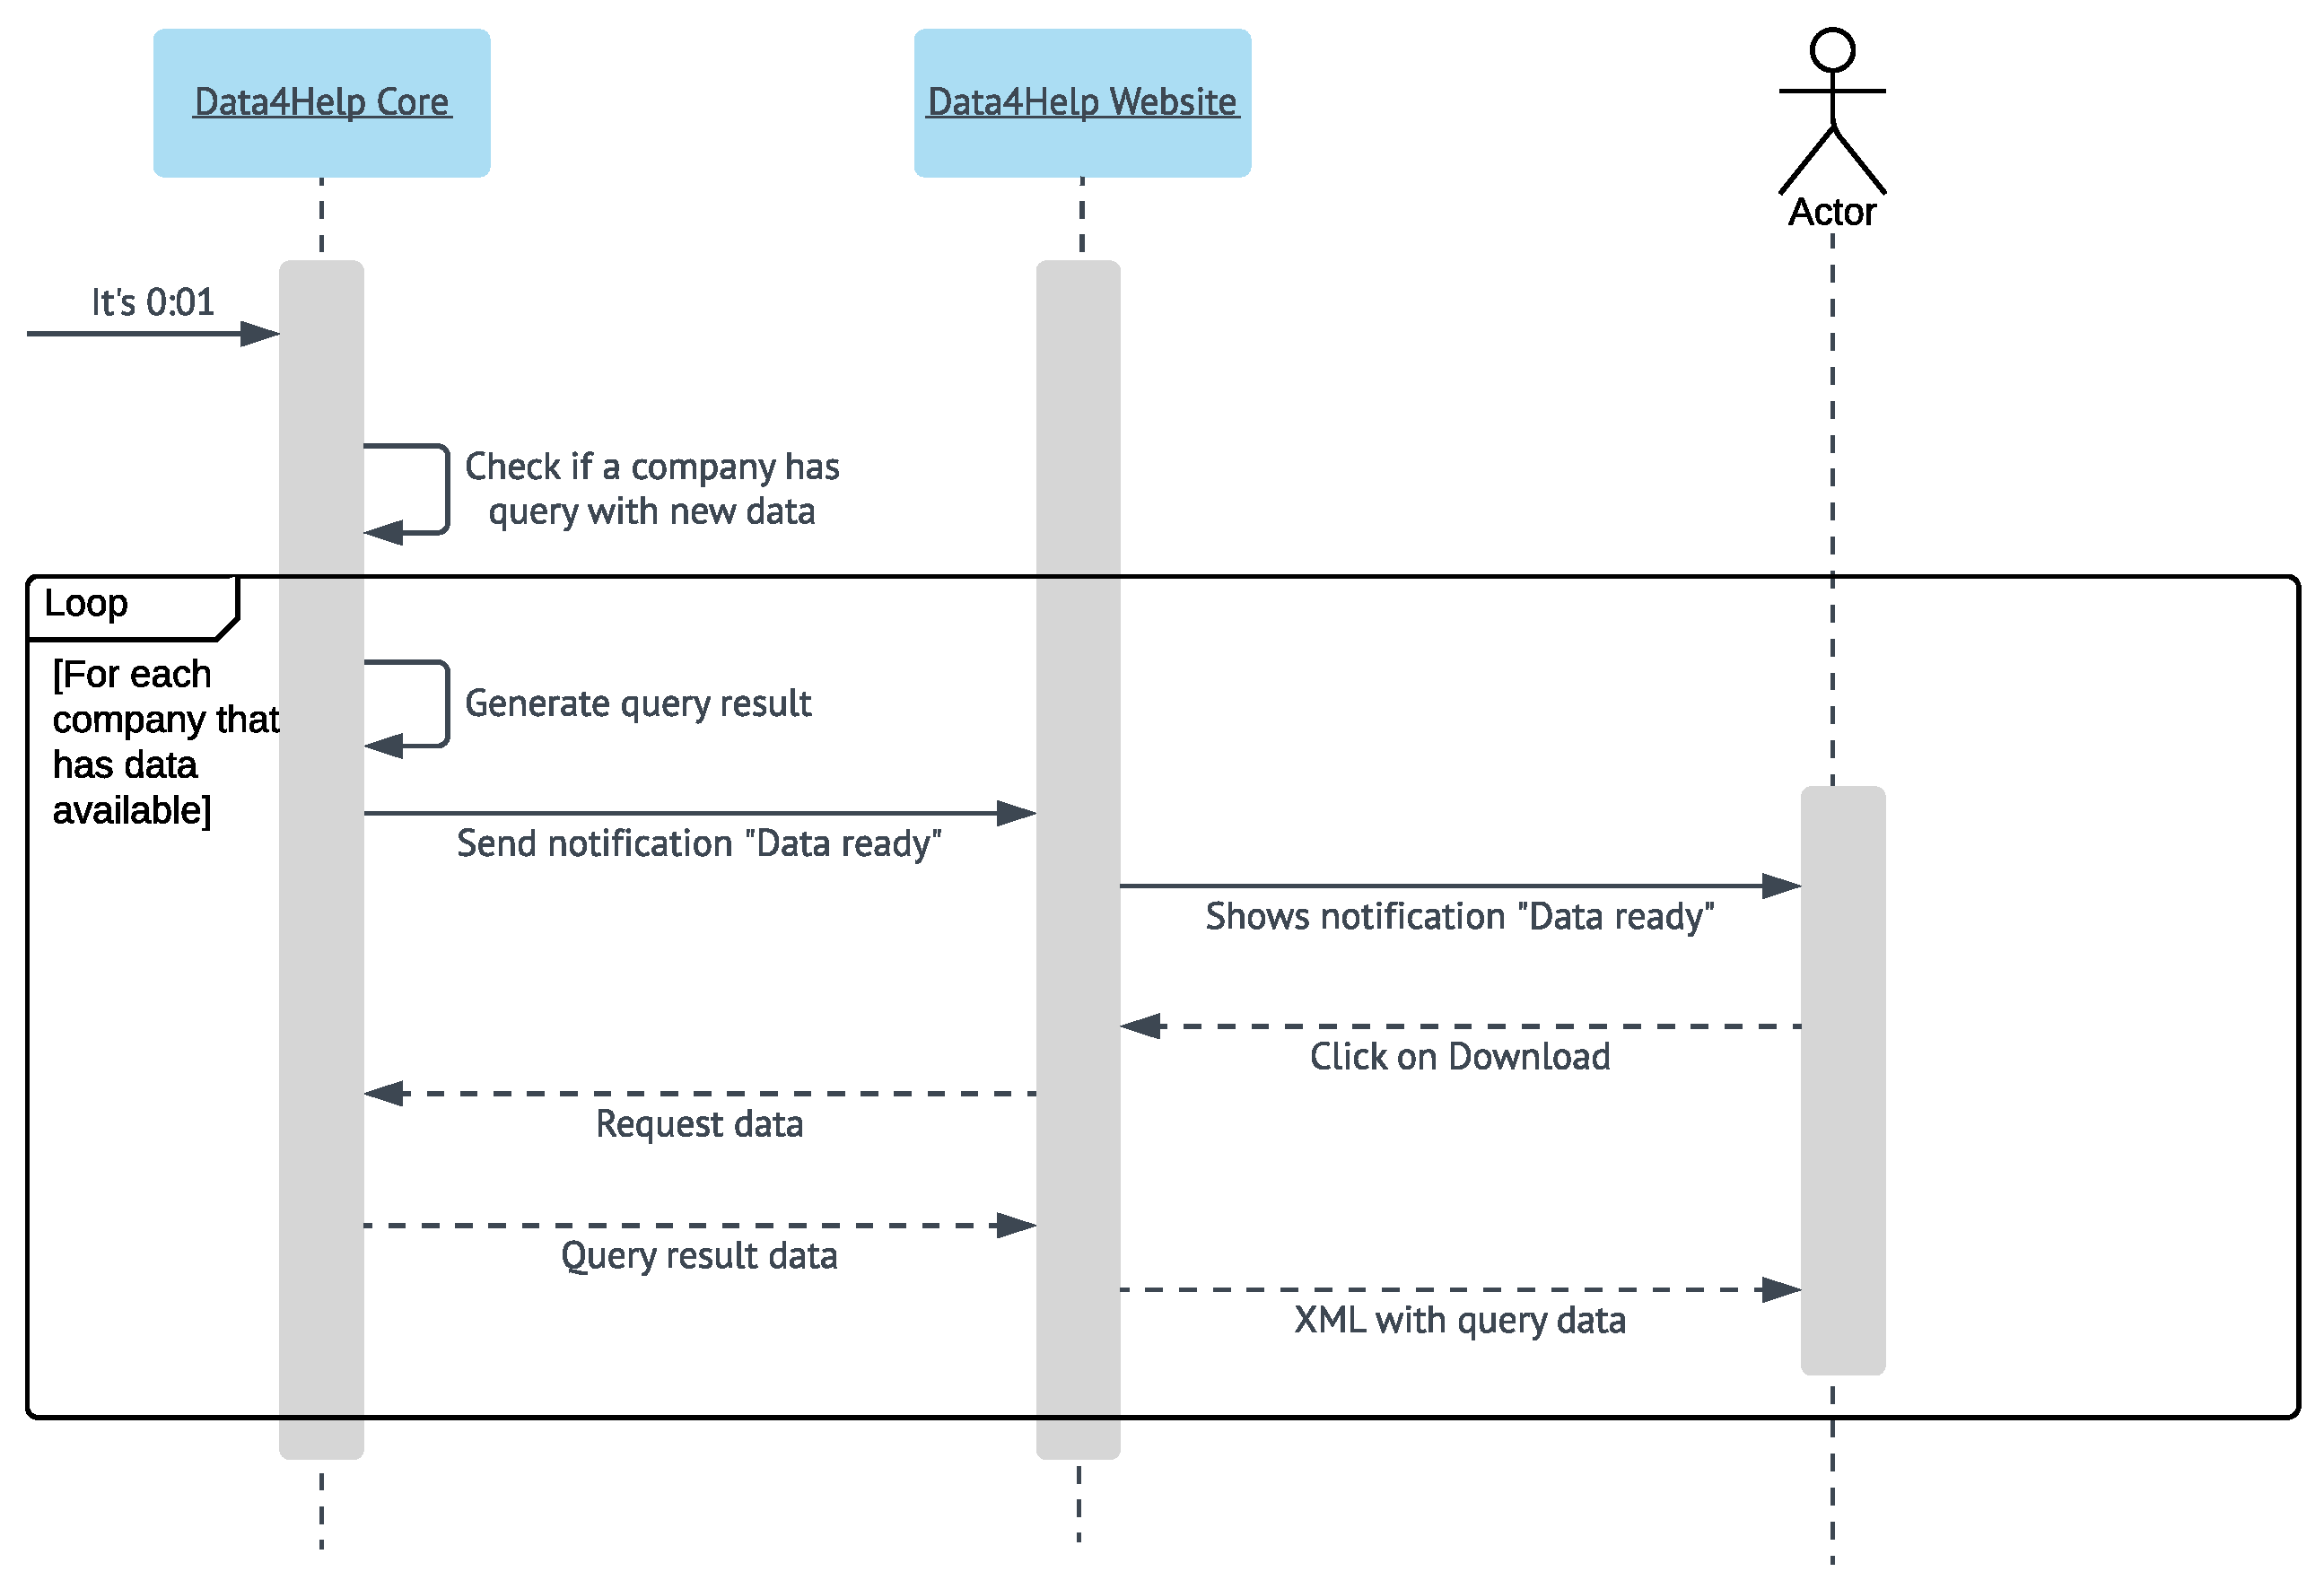
\includegraphics[width=\textwidth,height=\textheight,keepaspectratio]{assets/sequence/CompanyReceivesDataOfSubscribedQuery.pdf}
  \caption{Company receives data of subscribed query sequence diagram}
  \label{fig:CompanyReceivesDataOfSubscribedQuery}
\end{figure}

















\newpage
\paragraph{Emergency situation and ambulance call}
\begin{center}
\begin{table}[H]
\centering
\begin{tabular}{l|p{0.7\textwidth}}
\textbf{Actors} & User, core component \\
\textbf{Start conditions} & User health parameter under the threshold value \\
\textbf{Event flow}  & \begin{minipage}[t]{0.7\textwidth}
    \begin{itemize}
       \item System change the user status in “AMBULANCE NEED”
\item System connects hospital API 
\item Hospital API answer to the connection
\item System send emergency request to the hospital API sending location of the user and the health parameters under the threshold
\item Hospital API confirms that an ambulance has been sent to the position

    \end{itemize}
    
\end{minipage} \\
\textbf{Exit condition} & The user is labelled as “AMBULANCE SENT” \\
\textbf{Exceptions} & Hospital API refuses the connection \\
\textbf{Goals} & G9 
\end{tabular}

\end{table}
\end{center}
\begin{figure}[H]
  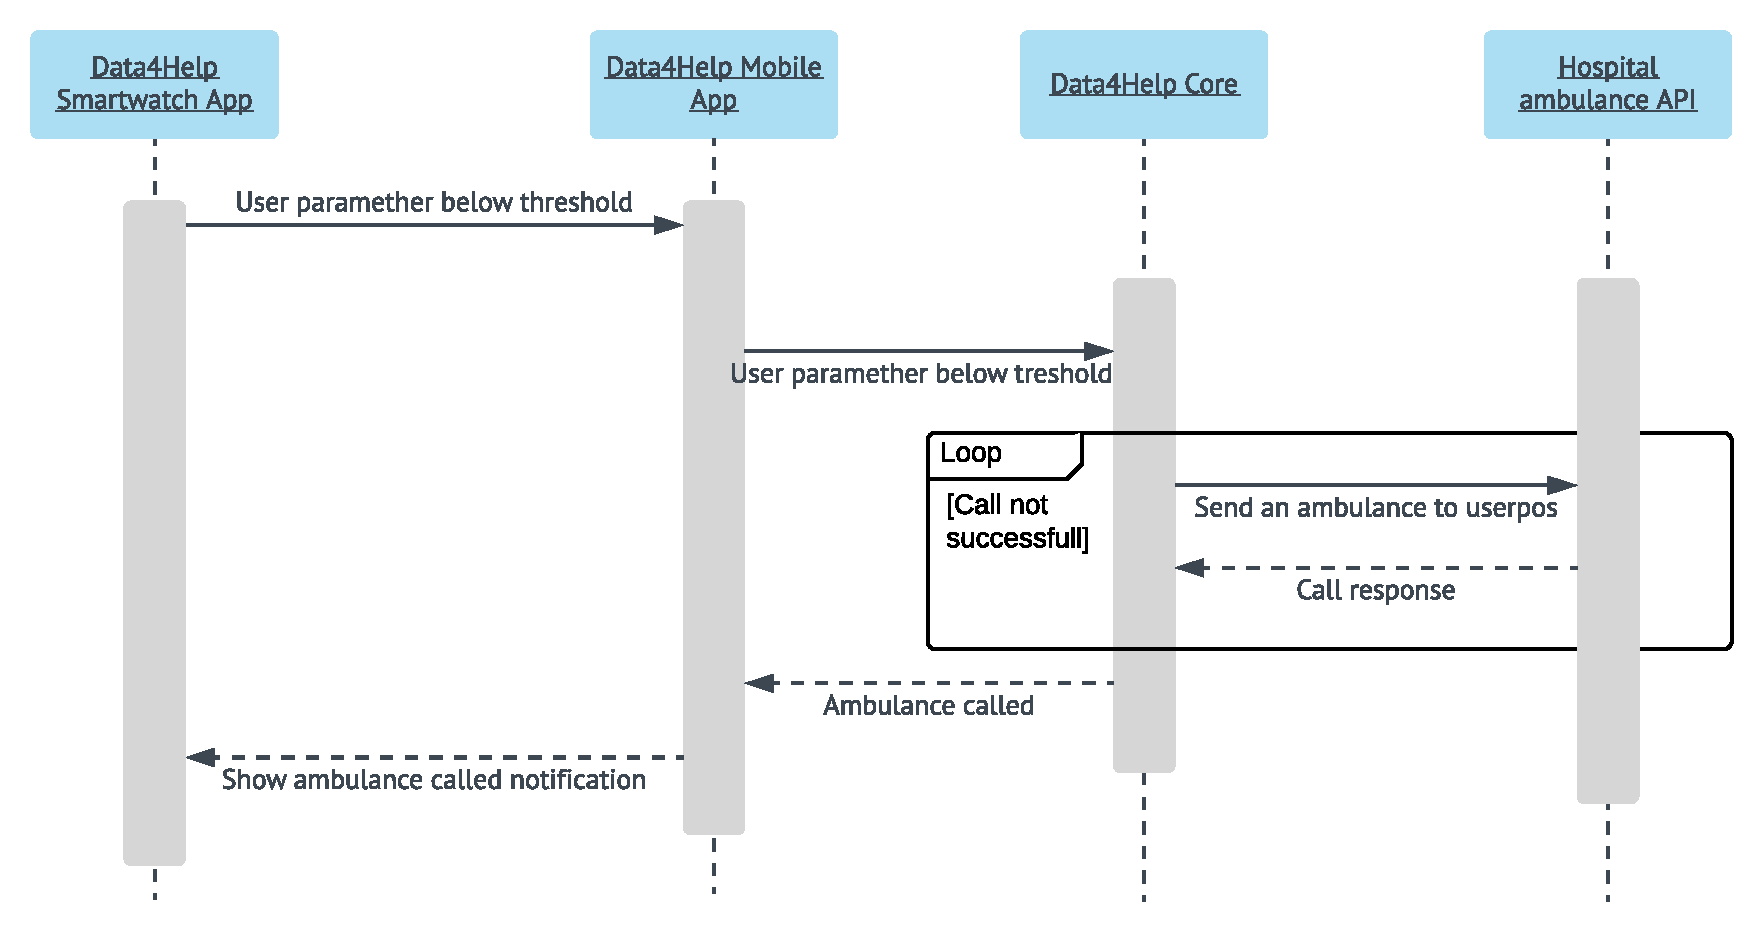
\includegraphics[width=\textwidth,height=\textheight,keepaspectratio]{assets/sequence/EmergencySituationAndAmbulanceCall.pdf}
  \caption{Emergency situation and ambulance call sequence diagram}
  \label{fig:EmergencySituationAndAmbulanceCall}
\end{figure}












\newpage
\paragraph{Run organizer registration}
\begin{center}
\begin{table}[H]
\centering
\begin{tabular}{l|p{0.7\textwidth}}
\textbf{Actors} & Not registered run organizer \\
\textbf{Start conditions} & None \\
\textbf{Event flow}  & \begin{minipage}[t]{0.7\textwidth}
    \begin{itemize}
       \item not registered company run organizer clicks on “Subscribe”
\item not registered run organizer inserts a username, an email and a password
\item The system checks if email is not used by any other user
\item The system generates a confirmation mail
\item The run organizer confirms the registration click on “Confirm email”
\item The system shows a registration complete screen


    \end{itemize}
    
\end{minipage} \\
\textbf{Exit condition} & Run organizer information used for registering is stored in the Data4Help database \\
\textbf{Exceptions} & \begin{minipage}[t]{0.7\textwidth}
    \begin{itemize}
       \item Not valid username
\item Not valid email
    \end{itemize}
    
\end{minipage} \\ \\
\textbf{Goals} & G10
\end{tabular}

\end{table}
\end{center}
\begin{figure}[H]
  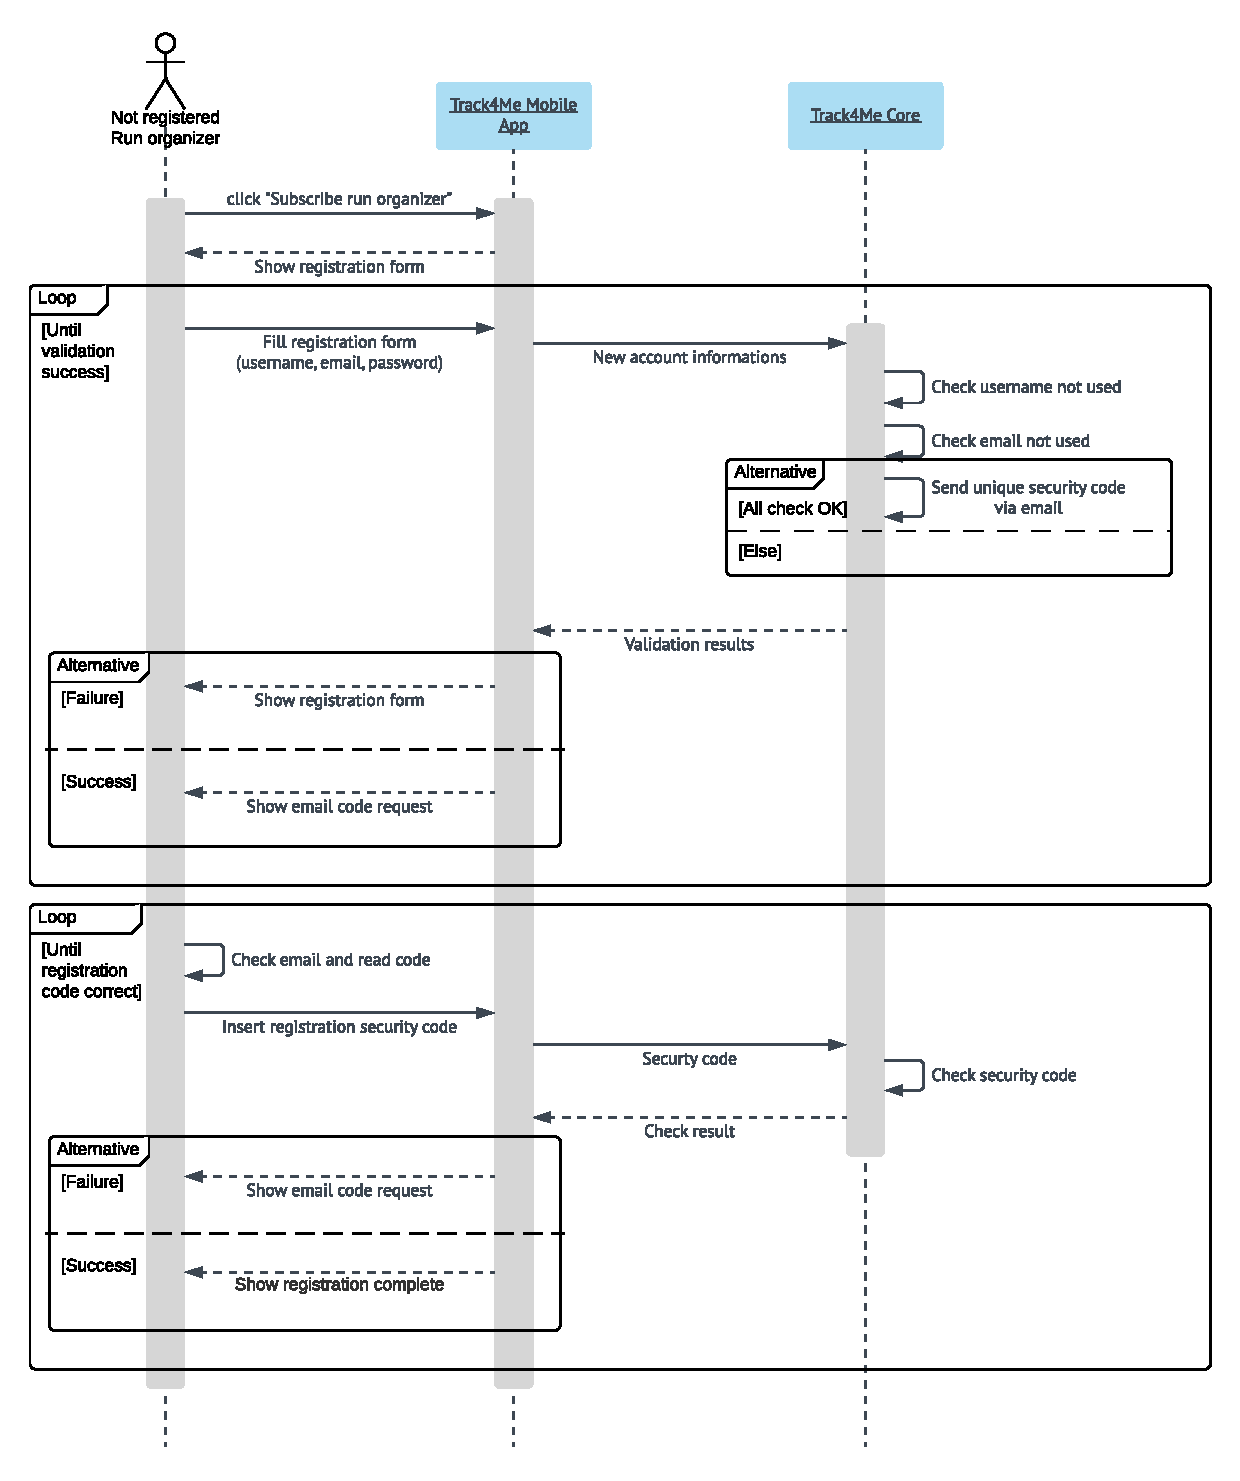
\includegraphics[width=\textwidth,height=\textheight,keepaspectratio]{assets/sequence/RunOrganizerRegistration.pdf}
  \caption{Run organizer registration sequence diagram}
  \label{fig:RunOrganizerRegistration}
\end{figure}















\newpage
\paragraph{Run organizer adds a new race}
\begin{center}
\begin{table}[H]
\centering
\begin{tabular}{l|p{0.7\textwidth}}
\textbf{Actors} & Run organizer \\
\textbf{Start conditions} & None \\
\textbf{Event flow}  & \begin{minipage}[t]{0.7\textwidth}
    \begin{itemize}
    \item Run organizer clicks on "Organize new run" on the Data4Help website 
    \item The system shows a screen with empty spaces about run information
    \item Run organizer insert the name of the run, the city where the run will take place, the date and the starting time
    \item The system checks if date is correct
    \item The system shows a map where user can define the path of the run
    \item Run organizer clicks on the path he wants the run to be taken
    \item The system calculates the km of the run
    \item The system show a "Correctly created run" screen
\end{itemize}
    
\end{minipage} \\
\textbf{Exit condition} & The system stores the information of the run in the Data4Help database and makes it public to users \\
\textbf{Exceptions} & \begin{minipage}[t]{0.7\textwidth}
    \begin{itemize}
\item Not valid date
    \end{itemize}
    
\end{minipage} \\ \\
\textbf{Goals} & G11
\end{tabular}

\end{table}
\end{center}

\begin{figure}[H]
  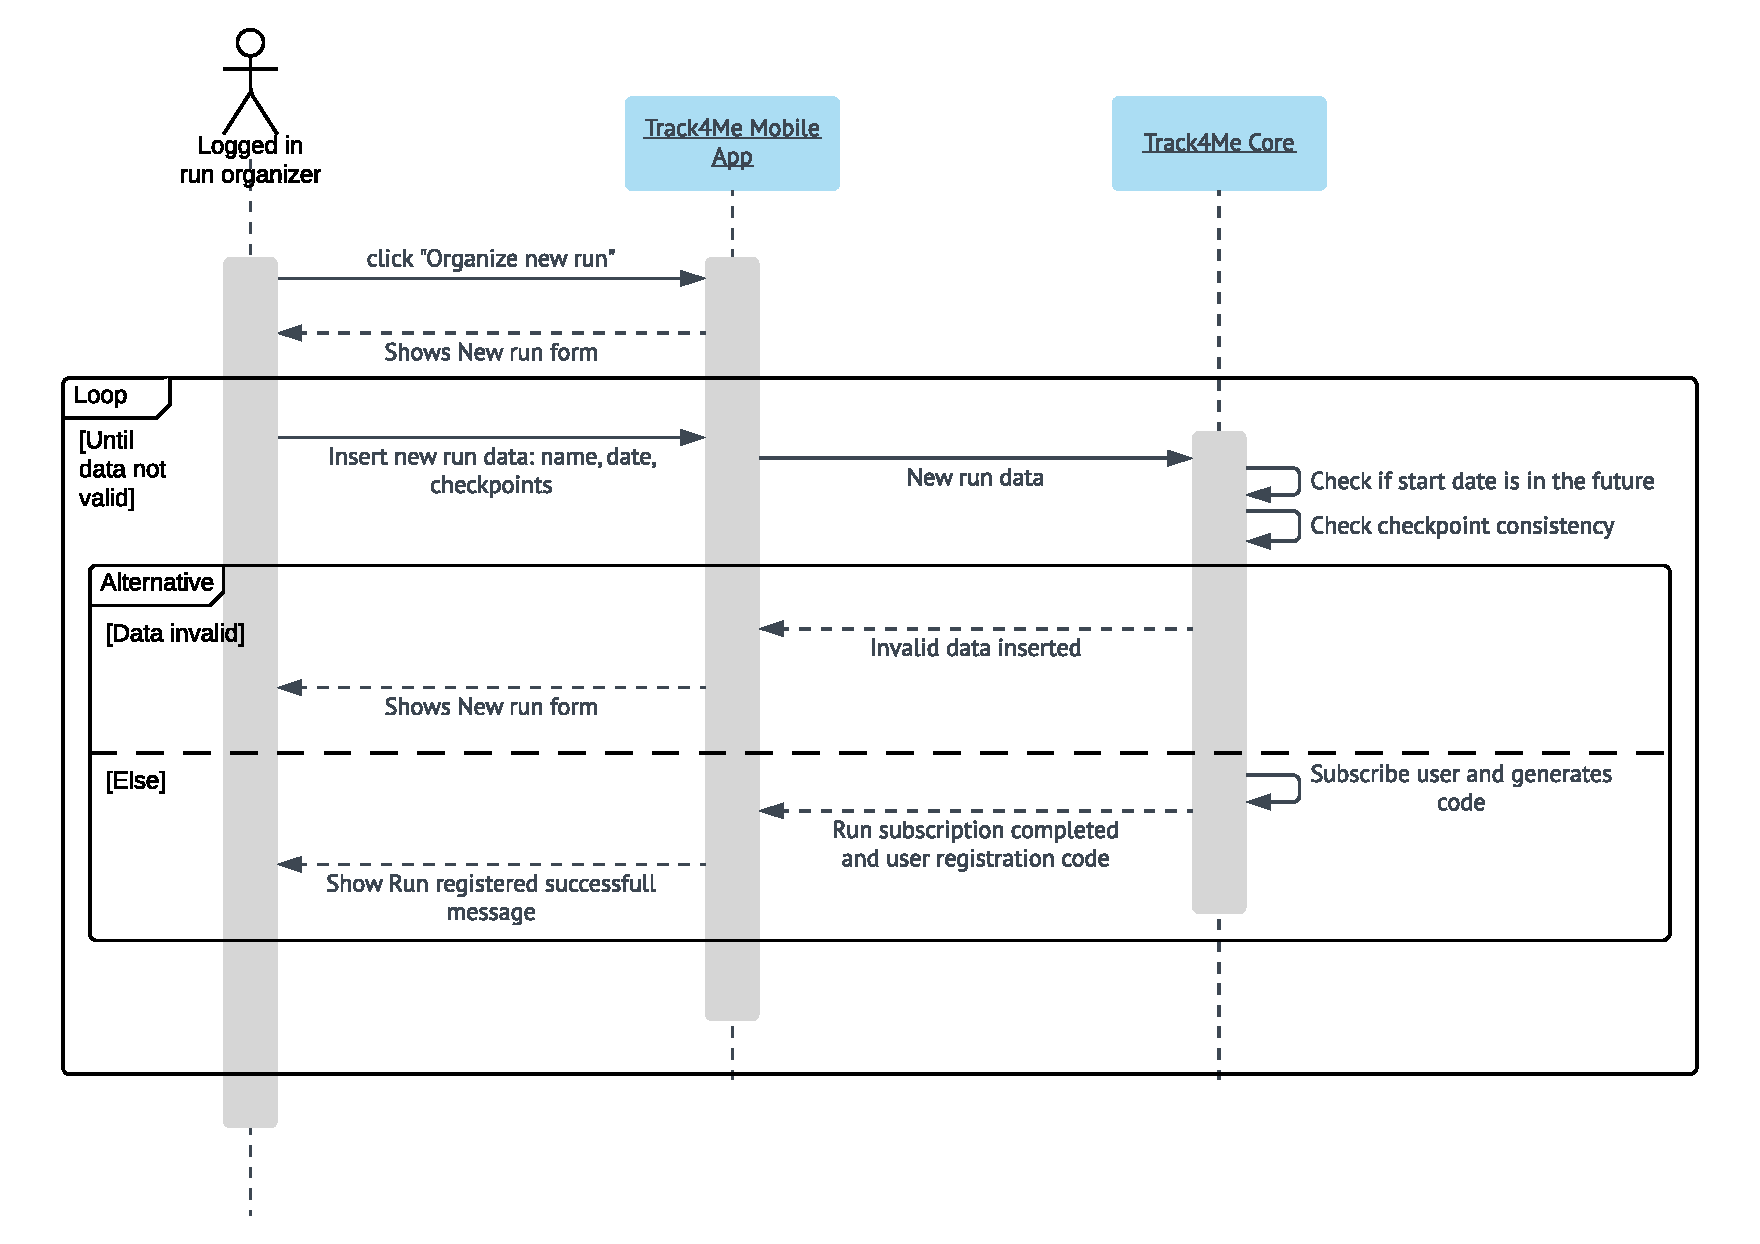
\includegraphics[width=\textwidth,height=\textheight,keepaspectratio]{assets/sequence/RunOrganizerAddsANewRace.pdf}
  \caption{Run organizer adds a new race sequence diagram}
  \label{fig:RunOrganizerAddsANewRace}
\end{figure}









\newpage
\paragraph{Runner subscription to a race}
\begin{center}
\begin{table}[H]
\centering
\begin{tabular}{l|p{0.7\textwidth}}
\textbf{Actors} & Run organizer\\
\textbf{Start conditions} & None \\
\textbf{Event flow}  & \begin{minipage}[t]{0.7\textwidth}
    \begin{itemize}
       \item Partecipant clicks on 'See nearby races'

        \item System shows a map with the races closer than 2 km from the user

\item Partecipant click on a run and clicks subscribe
\item The system verifies if it's still possible to subscribe

\item The system generates an runner ID number for the user
\item The system send the ID number to the user email
\item The user shows a correct subscription screenshot on the Mobile app

    \end{itemize}
    \end{minipage}
    \\
\textbf{Goals} & G12
\end{tabular}

\end{table}
\end{center}

\begin{figure}[H]
  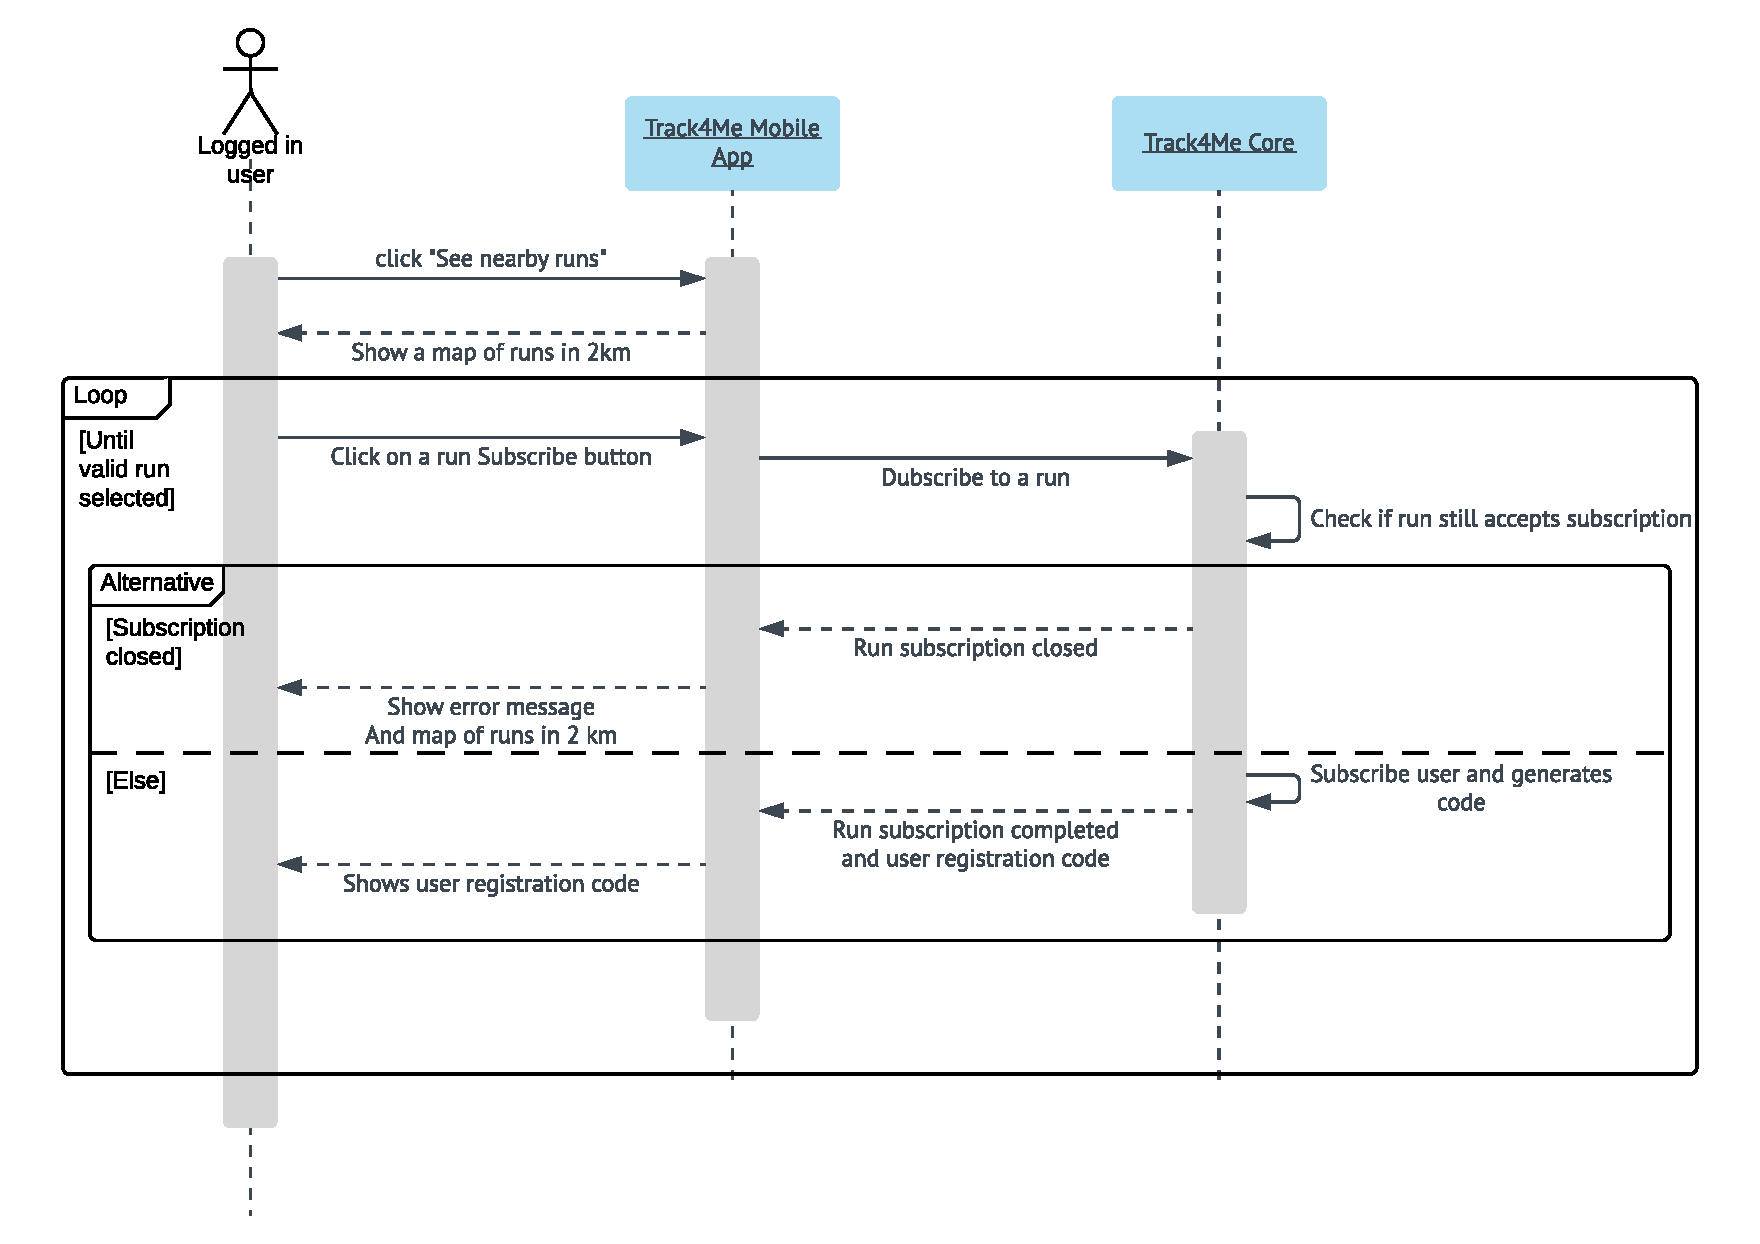
\includegraphics[width=\textwidth,height=\textheight,keepaspectratio]{assets/sequence/RunnerSubscriptionToARace.pdf}
  \caption{Runner subscription to a race sequence diagram}
  \label{fig:RunnerSubscriptionToARace}
\end{figure}







\newpage
\paragraph{Spectator or a run requests for runner position}
\begin{center}
\begin{table}[H]
\centering
\begin{tabular}{l|p{0.7\textwidth}}
\textbf{Actors} & User \\
\textbf{Start conditions} & None \\
\textbf{Event flow}  & \begin{minipage}[t]{0.7\textwidth}
    \begin{itemize}
       \item User clicks on "See nearby races"
\item System shows the map in radius of 2km from the user current position
\item User clicks on the desired run he wants to see and clicks on “see current runner positions”
\item The system shows a map with runners geographical position with their relative username and rank


    \end{itemize}
    
\end{minipage}  \\
\textbf{Exit condition} & None \\
\textbf{Exceptions} & \begin{minipage}[t]{0.7\textwidth}
    \begin{itemize}
       \item Run has already finished
\item Run hasn't already started


    \end{itemize}
    
\end{minipage}  \\
\textbf{Goals} & G13 
\end{tabular}

\end{table}
\end{center}

\begin{figure}[H]
  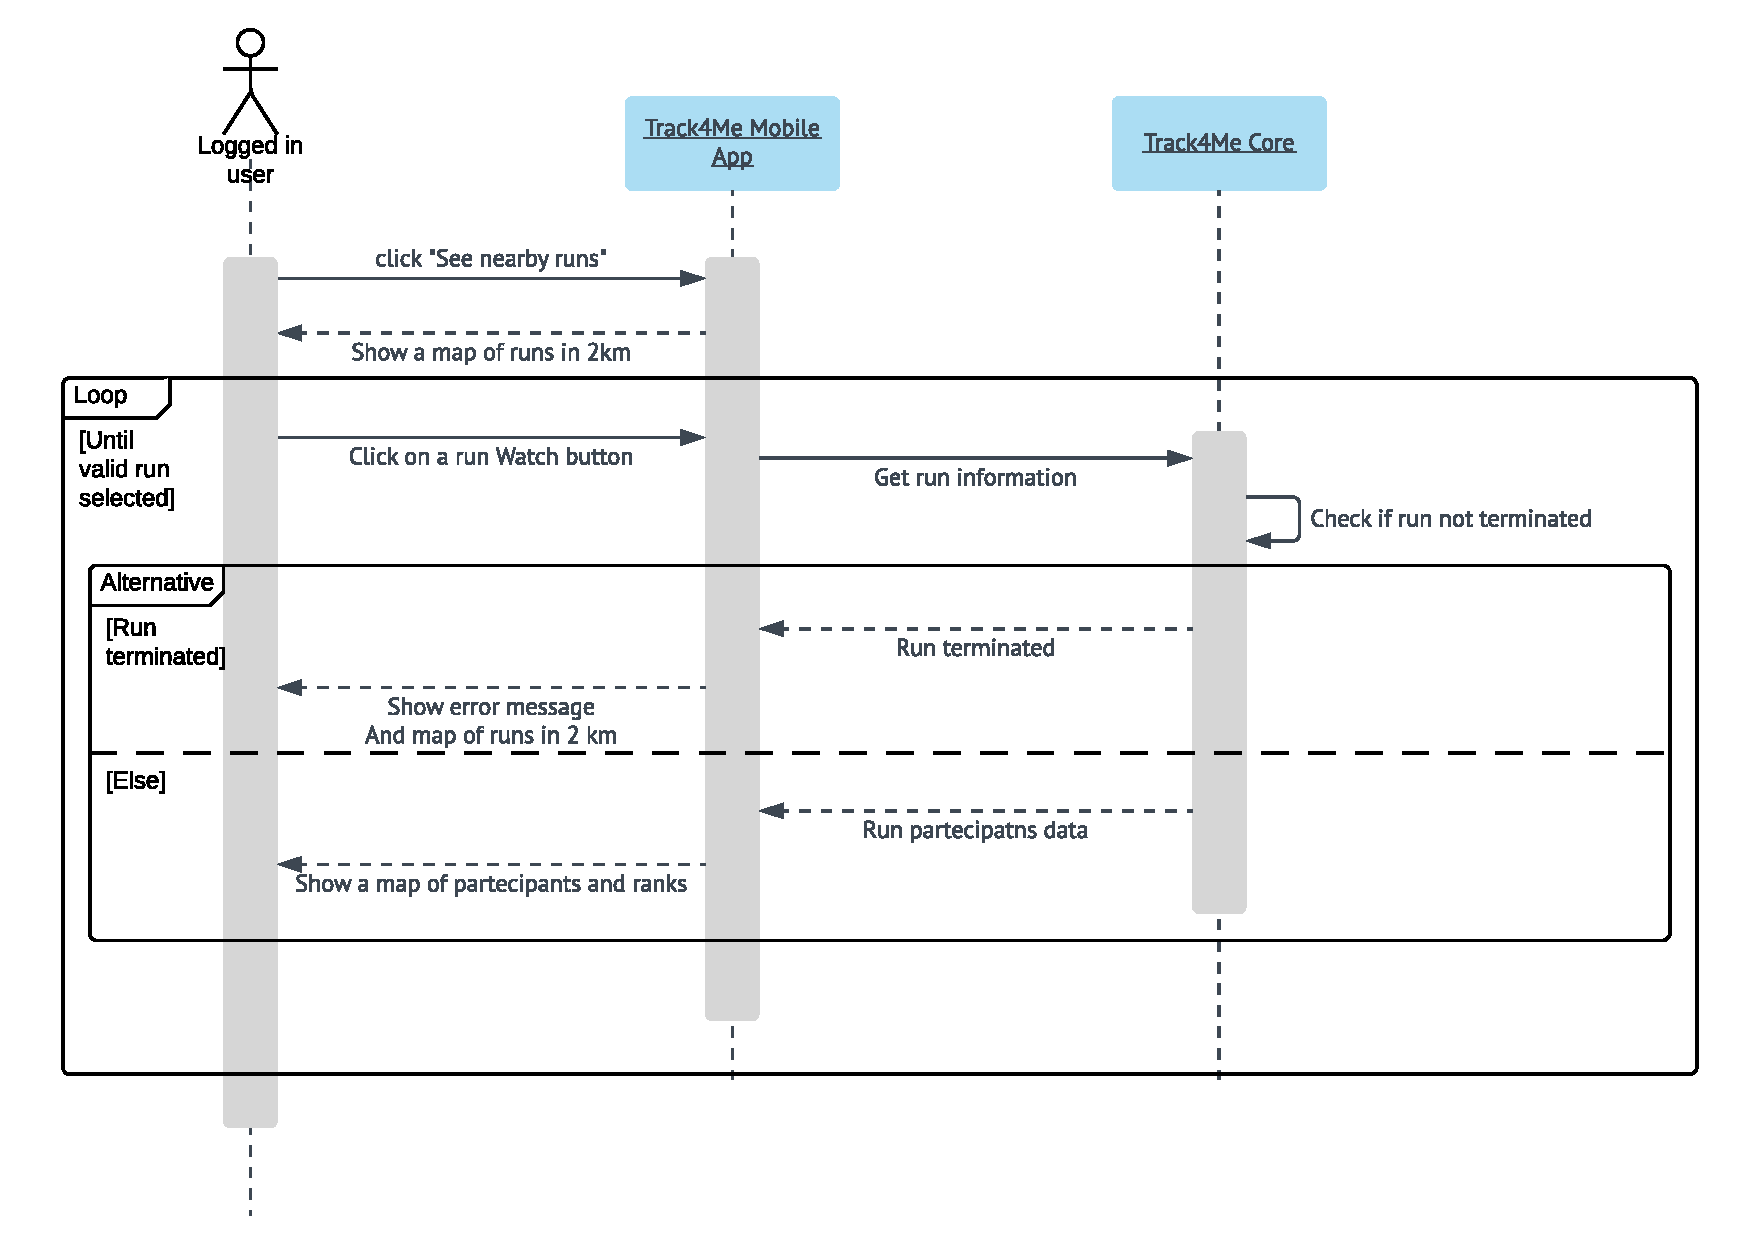
\includegraphics[width=\textwidth,height=\textheight,keepaspectratio]{assets/sequence/SpectatorOfARunRequestsForRunnerPosition.pdf}
  \caption{Spectator or a run requests for runner position sequence diagram}
  \label{fig:SpectatorOfARunRequestsForRunnerPosition}
\end{figure}

